\documentclass[10pt,draft]{beamer}

\usetheme[progressbar=frametitle]{metropolis}
\usepackage{appendixnumberbeamer}

\usepackage{booktabs}
\usepackage[scale=2]{ccicons}

% \usepackage{xspace}
% \newcommand{\themename}{\textbf{\textsc{metropolis}}\xspace}

%%% MATHS
\usepackage{amsmath,amsfonts,amsthm}
\usepackage{siunitx}
\sisetup{range-units=single, range-phrase=--}
\usepackage{cool}

%%% FONTS
\usepackage[normalem]{ulem}

\usepackage{fontawesome}
\newcommand{\emailsymbol}   {\faEnvelope~~}  % alternative: \faInbox
\newcommand{\homepagesymbol}{\faGlobe~~}  % alternative: \faHome
\newcommand{\twittersymbol} {\faTwitter~~}
\newcommand{\githubsymbol}  {\faGithub~~}

%%% COLOURS
\usepackage{xcolor}
\definecolor{C0}{HTML}{1F77B4}
\definecolor{C1}{HTML}{FF7F0E}

%%% MISC
\usepackage{datetime}

%%% TABLES
\usepackage{booktabs}
\usepackage{tabularx}

%%% THEME SETTINGS
\setbeamertemplate{frame footer}{\tiny{NORPAN workshop 2017}}

%%% TITLE
\title{The influence of surface conditions on polar low generation near Svalbard archipelago}
\subtitle{\small{NORPAN Workshop on Atmosphere-Ice-Ocean Interactions}}
\date{\today}
\author{\textbf{Denis Sergeev}, Ian Renfrew, Thomas Spengler}
\titlegraphic{%

\includegraphics[height=1.0cm]{{logos/uealogo}.png}\hfill

\includegraphics[height=1.0cm]{{logos/coaslogo}.png}\hfill

\includegraphics[height=1.0cm]{{logos/bergenlogo}.png}\hfill
}

\hypersetup{
pdfauthor = {Denis Sergeev: d.sergeev@uea.ac.uk},
pdfsubject = {Slides for NORPAN workshop},
pdfkeywords = {polar lows, sea ice, orography, MetUM, Arctic, Svalbard},
pdfmoddate= {D:\pdfdate},
pdfcreator = {}
}

% \usepackage[left=2cm,
%             right=2cm,
%             top=2cm,
%             bottom=2cm,
%             headheight=1cm
%            ]{geometry}

\begin{document}

\maketitle

% \begin{frame}{Table of contents}
%   \setbeamertemplate{section in toc}[sections numbered]
%   \tableofcontents[hideallsubsections]
% \end{frame}

\section{Introduction}
\begin{frame}{\sout{Fantastic beasts} Polar lows and where to find them}
\begin{itemize}
\item \textit{Polar lows} are small (\SIrange{100}{500}{\km} in diameter), short-lived maritime depressions with near-surface winds exceeding \SI{15}{\meter\per\s}
\item They develop in the regions prone to \alert{CAOs}, where relatively cold continental air is advected over warm ice-free waters
\end{itemize}
\begin{center}
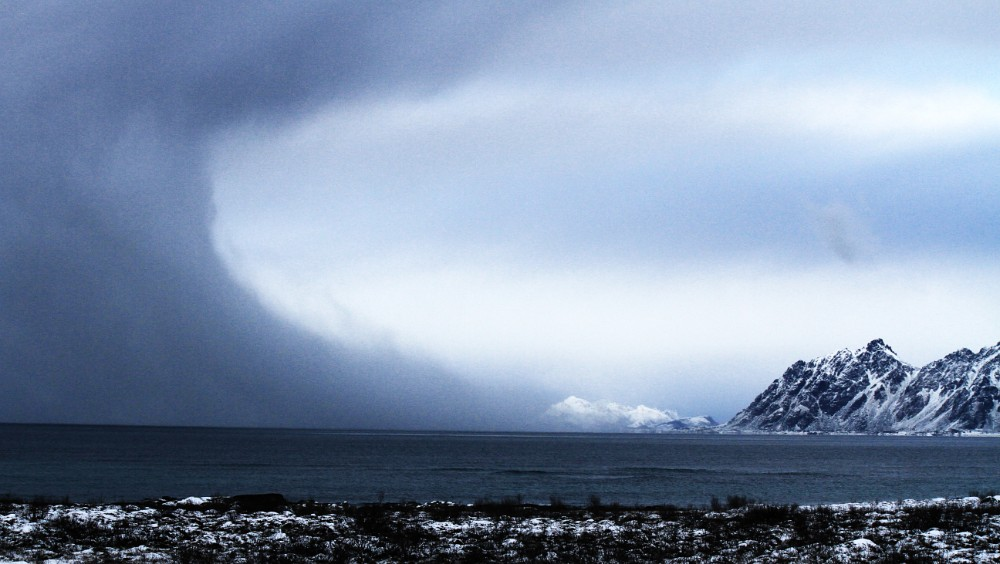
\includegraphics[width=0.7\textwidth]{{figures/PL_19122014_Lofoten}.jpg}\\
\tiny A polar low near Lofoten Islands (\href{http://www.nrk.no/nordland/polart-lavtrykk-inn-mot-nordland-natt-til-sondag-1.12112660}{NRK.no})
\end{center}
\end{frame}


\begin{frame}{Surface conditions}
\begin{columns}
\begin{column}{0.5\textwidth}
\underline{Hypothesis 1}:\\
Svalbard's \alert{orography} deflects the northerly flow\\
$$\Downarrow$$
Let's remove Svalbard!\\{\small (Replace it with sea ice)}
\end{column}
\begin{column}{0.5\textwidth}
\underline{Hypothesis 2}:\\
\alert{Sea ice} extent defines where polar lows develop\\
$$\Downarrow$$
Let's change the sea ice edge!
\end{column}
\end{columns}
\end{frame}

\begin{frame}{Motivation}
\begin{itemize}
\item
Hardly any research focused on the Svalbard as a \alert{trigger mechanism} for polar lows
\item
Sea ice configuration is crucial for \alert{convergence zone} and its evolution into a cyclone
\item
Will location and impact of polar lows change with different sea conditions in the \alert{warming climate}?
\end{itemize}
\begin{columns}
\begin{column}{0.3\textwidth}
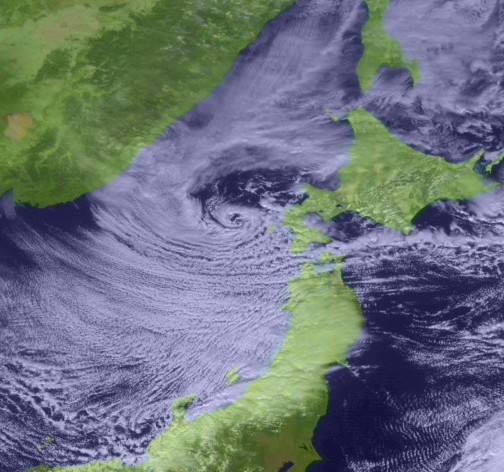
\includegraphics[width=\textwidth]{{figures/pl_japansea}.jpg}\\
{\tiny Source: \href{http://www.atmos.rcast.u-tokyo.ac.jp/hotspot/eng/selected2/a01_k1.html}{U. Tokyo}}
\end{column}
\begin{column}{0.3\textwidth}
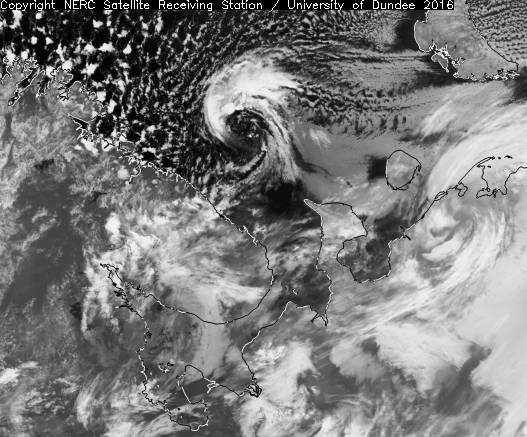
\includegraphics[width=\textwidth]{{figures/polarlow_barentssea}.jpg}\\
{\tiny Source: \href{http://www.sat.dundee.ac.uk/}{NERC Satellite Receiving Station}}
\end{column}
\begin{column}{0.3\textwidth}
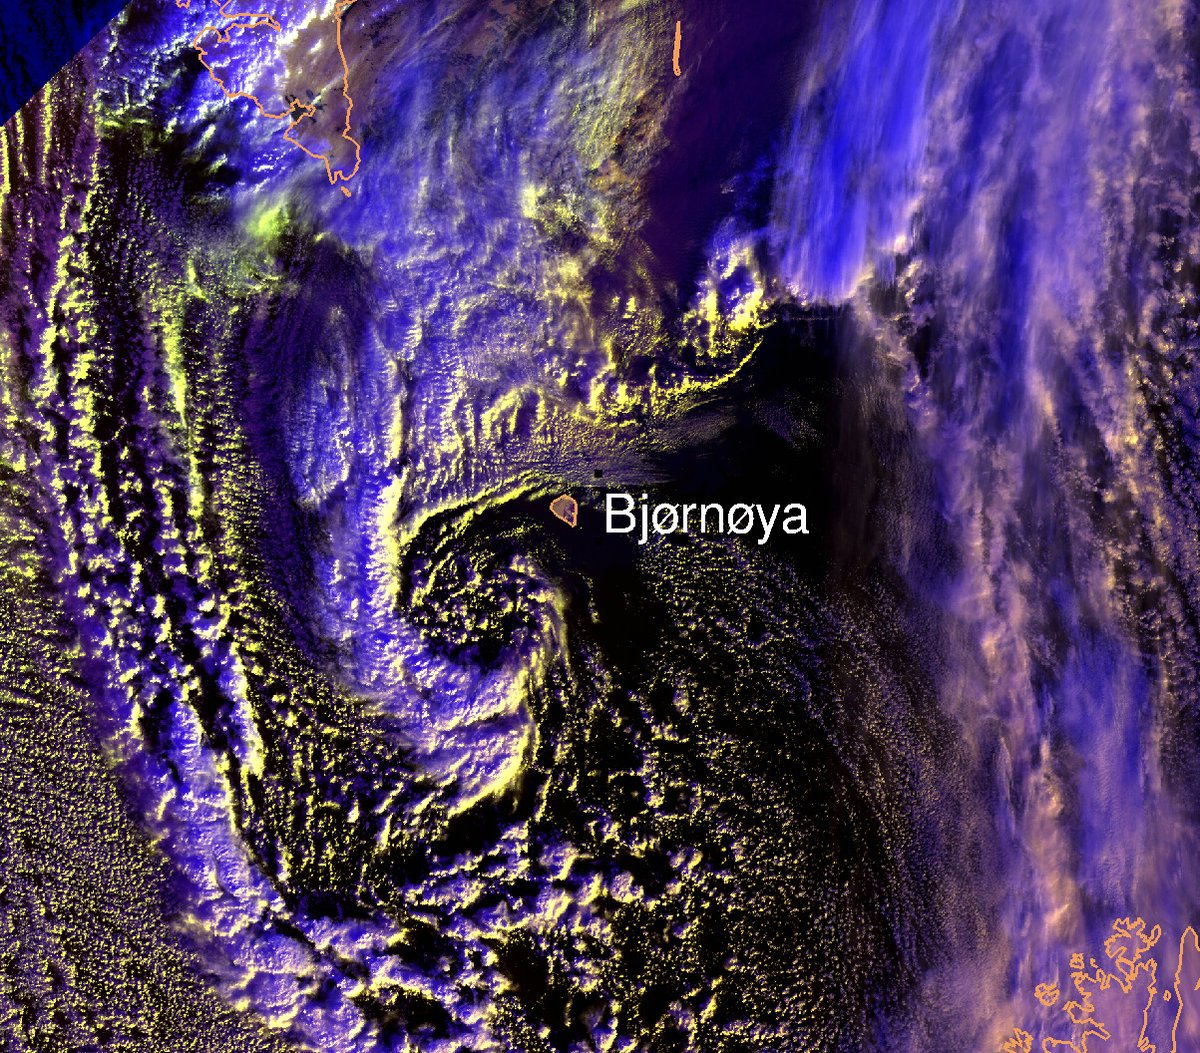
\includegraphics[width=\textwidth]{{figures/polarlow_metno}.jpg}\\
{\tiny Source: \href{https://twitter.com/Meteorologene}{MET Norway}}
\end{column}
\end{columns}
\end{frame}

\section{Data and methods}
\begin{frame}{Model set-up}
\begin{columns}
\begin{column}{0.5\textwidth}
{\small
\begin{table}
\caption{Met Office Unified model parameters (nested domain)}
\begin{tabularx}{\textwidth}{ll}
\toprule
Version & 10.2 \\
Horizontal grid spacing & \SI{2.2}{\kilo\meter}\\
Number of grid points & $600\times 700$\\
% Nested domain area & \SI{1320}{\kilo\meter}$\times$ \SI{1540}{\kilo\meter}\\
Nested domain centre & \ang{76}N \ang{10}E \\
Run duration & \SI{48}{\hour}\\
Output frequency & \SI{1}{\hour}\\
\bottomrule
\end{tabularx}
\end{table}
}
\end{column}
\begin{column}{0.5\textwidth}
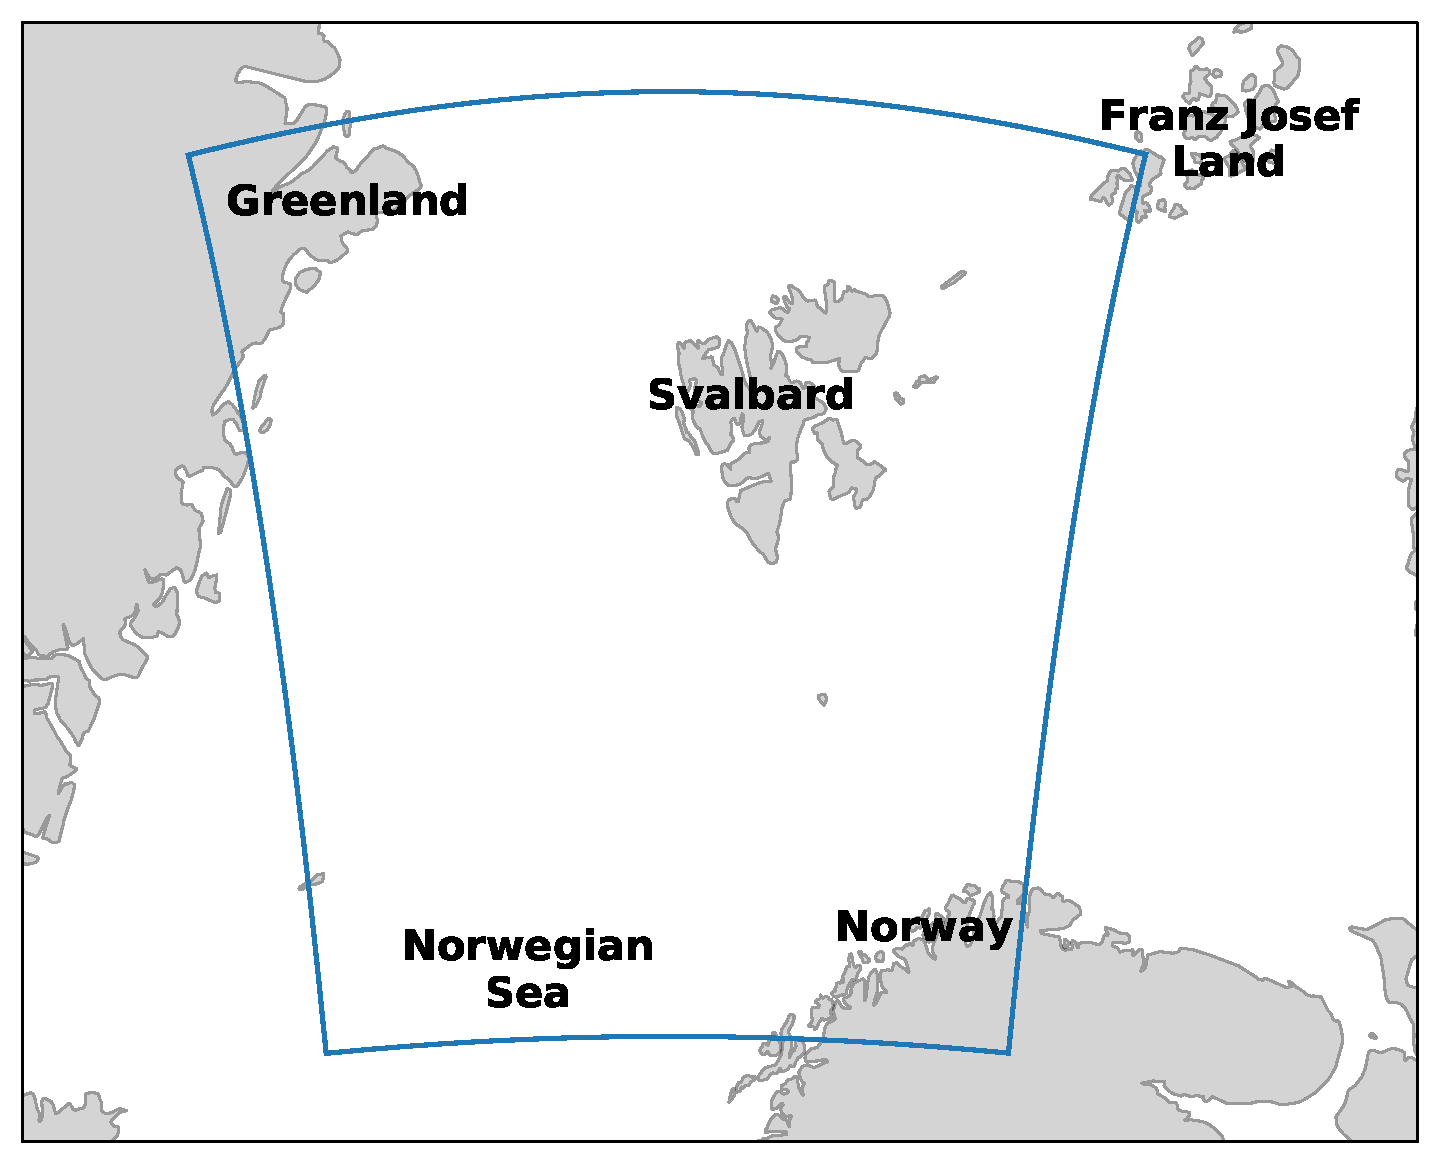
\includegraphics[width=\textwidth]{{figures/model_domain}.pdf}
\end{column}
\end{columns}
\end{frame}

\begin{frame}{Polar low cases}
\begin{itemize}
\item We use STARS database (\href{http://polarlow.met.no}{http://polarlow.met.no})
\item 7 most interesting polar low cases have been simulated
\item Chosen by their \alert{southward propagation} and \alert{proximity to Svalbard}.
\end{itemize}
\end{frame}

\begin{frame}{Polar low cases: control run}
\begin{center}
TOA OLR (cloud pattern); SLP contours; precipitation rate\\
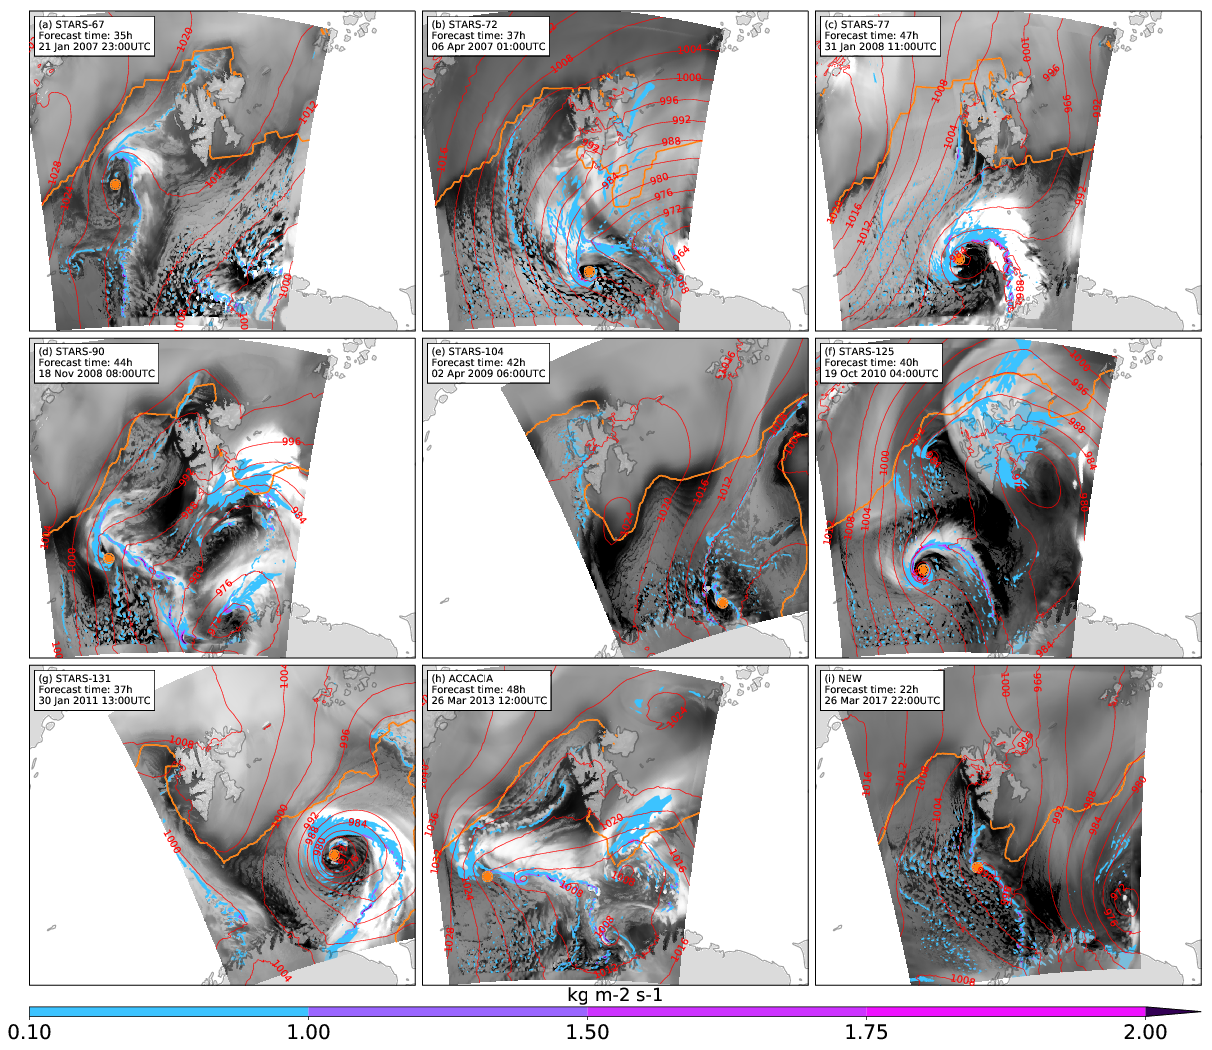
\includegraphics[width=0.8\linewidth]{{figures/lwtoa_seaice_snowrate_slp_max_ke_ctrl}.png}
\end{center}
\end{frame}

\begin{frame}{ACCACIA polar low}
\begin{itemize}
\item Analysed extensively using aircraft and satellite observations
\item Used for validation of the Met Office model
\end{itemize}
\begin{columns}
\begin{column}{0.4\textwidth}
\begin{itemize}
\item The model reproduces well the strength of the \alert{horizontal wind shear}, and temperature and humidity gradient
\item The model \alert{underestimated the liquid water} content and height of the cloud layers
\end{itemize}
\end{column}
\begin{column}{0.6\textwidth}
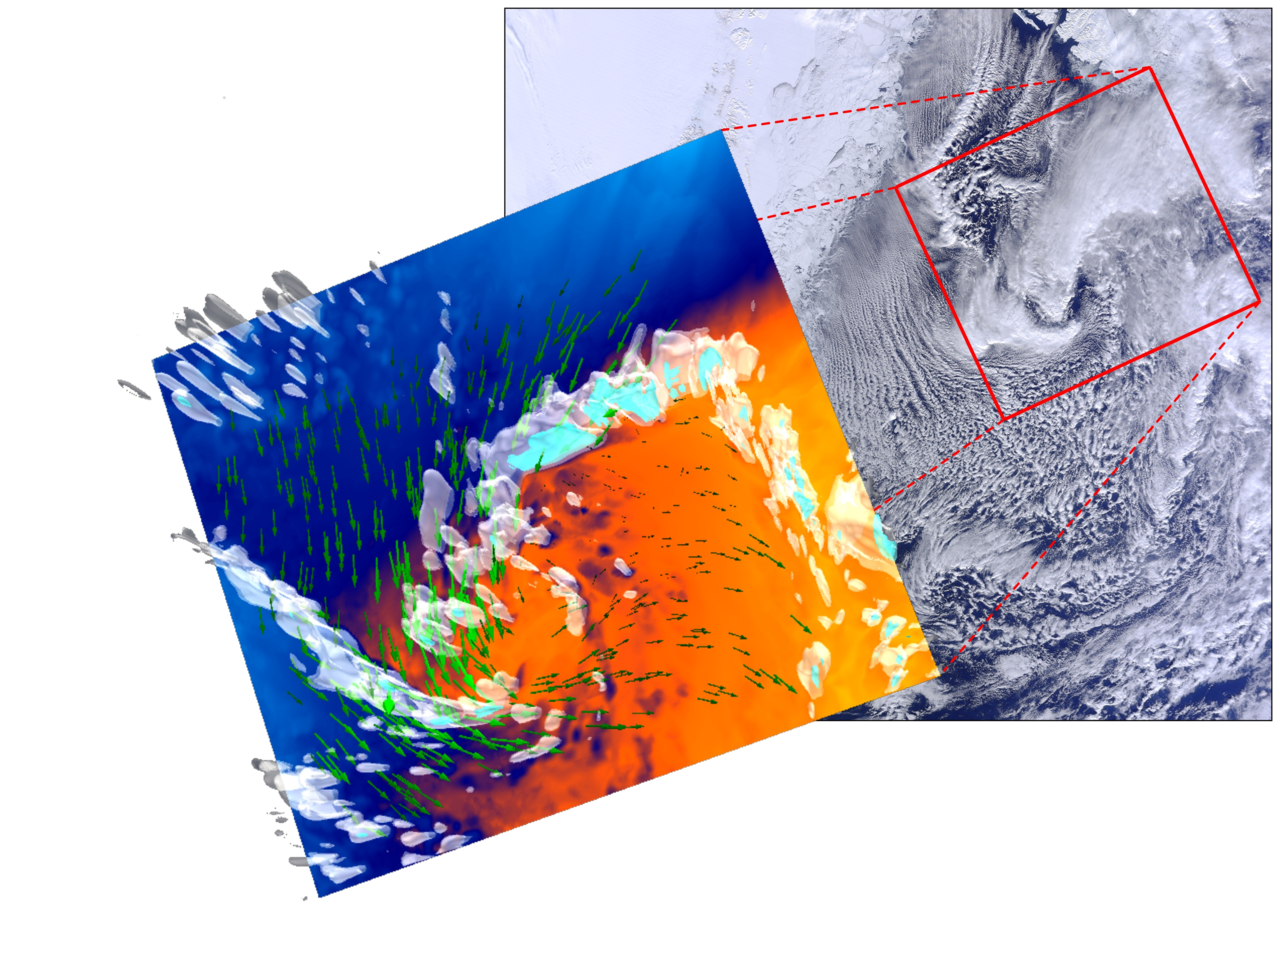
\includegraphics[width=\textwidth]{{figures/featured_image_lowres}.png}
\end{column}
\end{columns}
\end{frame}

\begin{frame}{ACCACIA polar low}
\begin{center}
More info in this paper [Sergeev et al., 2017]:\\
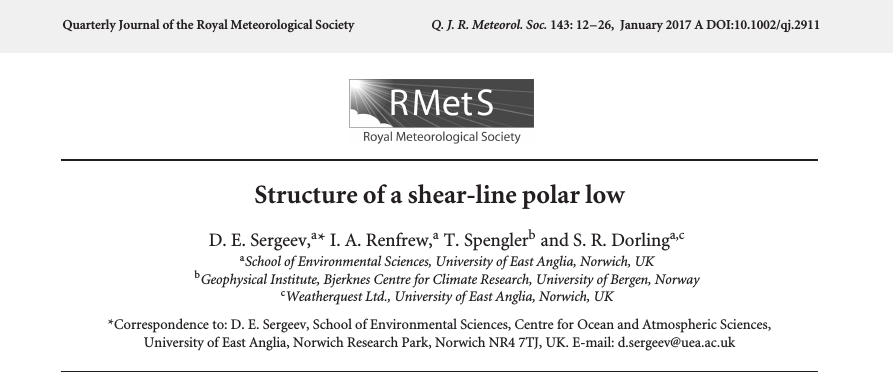
\includegraphics[width=\textwidth]{{figures/paper}.png}\\
\small Don't be shy to cite!
\end{center}
\end{frame}

\begin{frame}{Sensitivity experiments}
\begin{center}
SST, sea ice, and orography configuration
\par
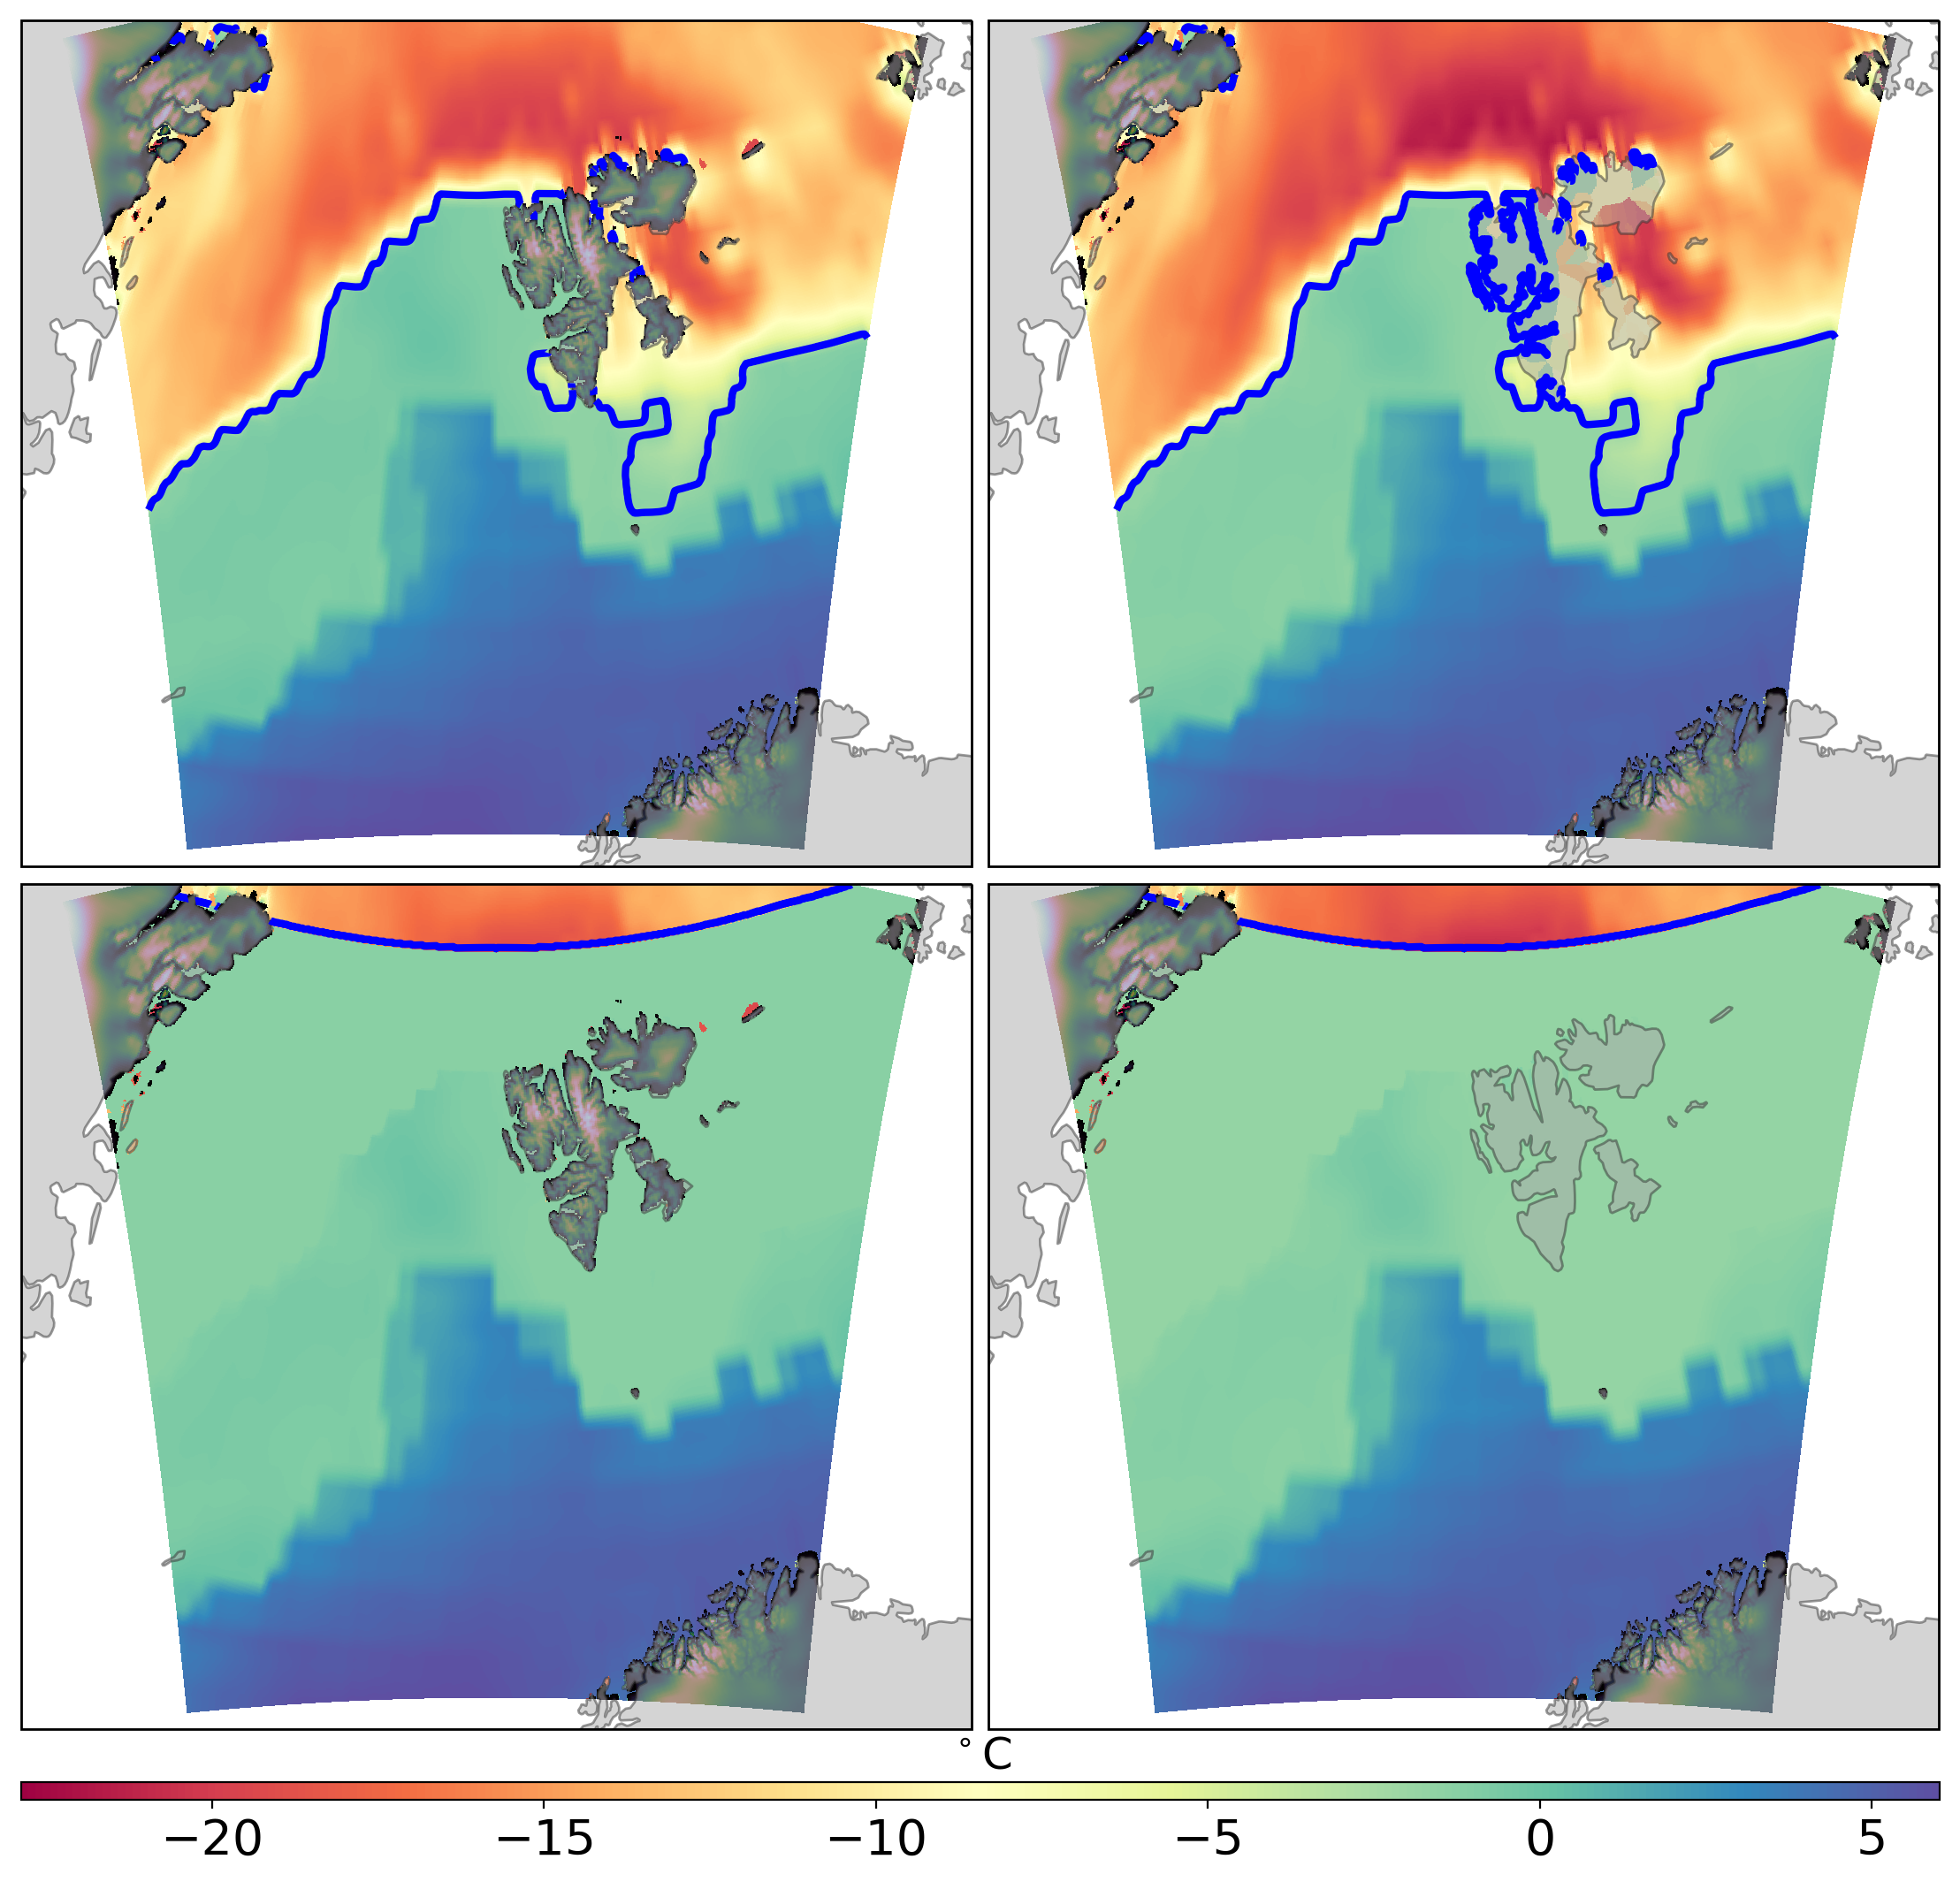
\includegraphics[width=0.7\textwidth]{{figures/surftemp_orog_seaice}.png}
\end{center}
\end{frame}

\section{Results}
\begin{frame}{Polar low tracks}
\begin{center}
Manually tracked polar low paths in the \textcolor{C0}{control} and \textcolor{C1}{perturbed} runs\par
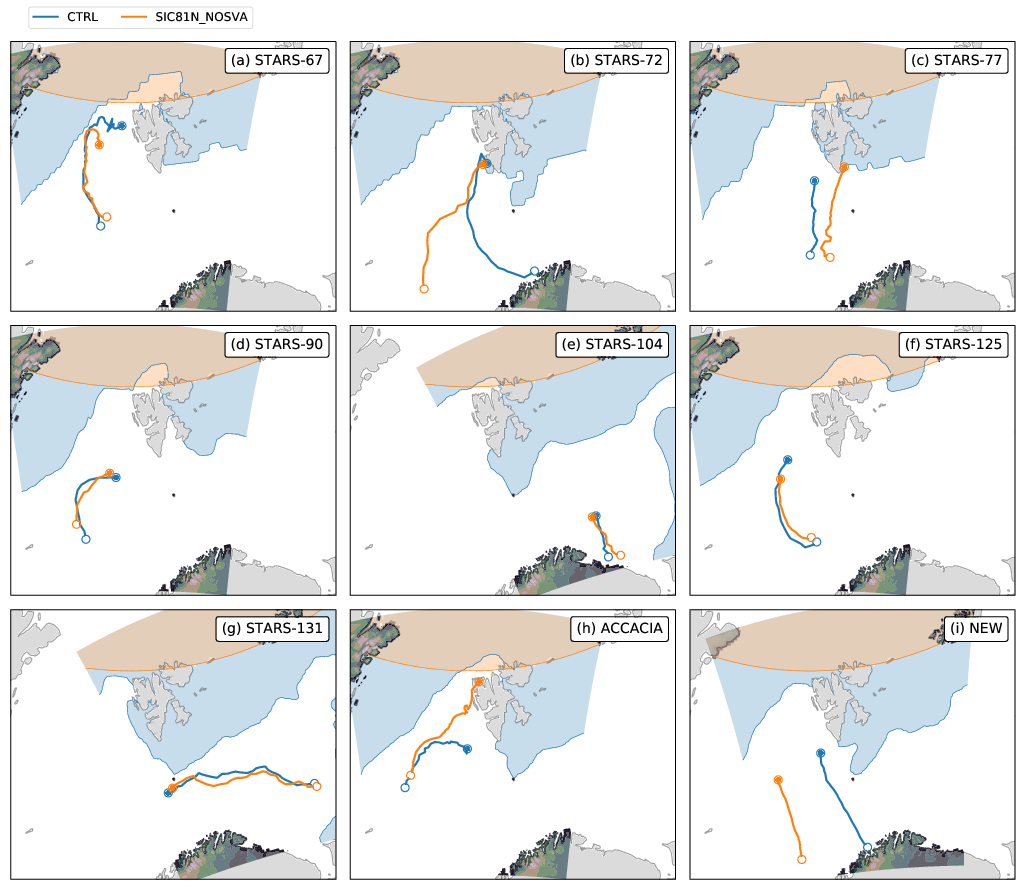
\includegraphics[width=0.7\textwidth]{{figures/all_pl_tracks_ctrl_sic81n_nosva}.pdf}
\end{center}
\end{frame}

\begin{frame}{Structure overview}
\begin{center}
Cyclonic vorticity at \SI{950}{hPa} above the threshold of \SI{e-3}{\per\second} in the \textcolor{C0}{control} and \textcolor{C1}{perturbed} runs\par
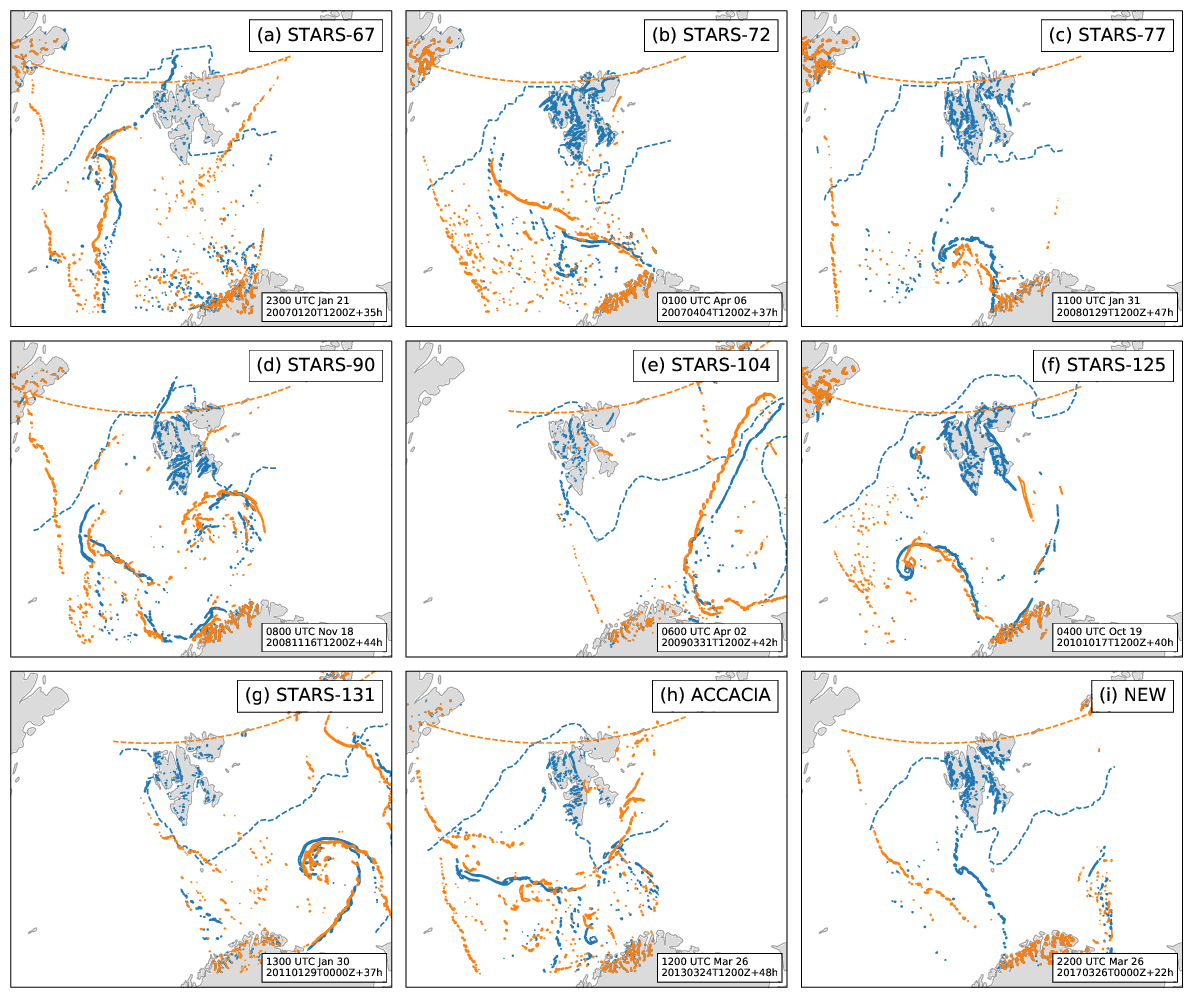
\includegraphics[width=0.7\textwidth]{{figures/all_pl_vort_ctrl_sic81n_nosva}.pdf}
\end{center}
\end{frame}

\section{Focus on STARS-72 polar low case}
\begin{frame}{STARS-72 polar low}
\begin{center}
AVHRR IR image of polar low event at one selected time
\par
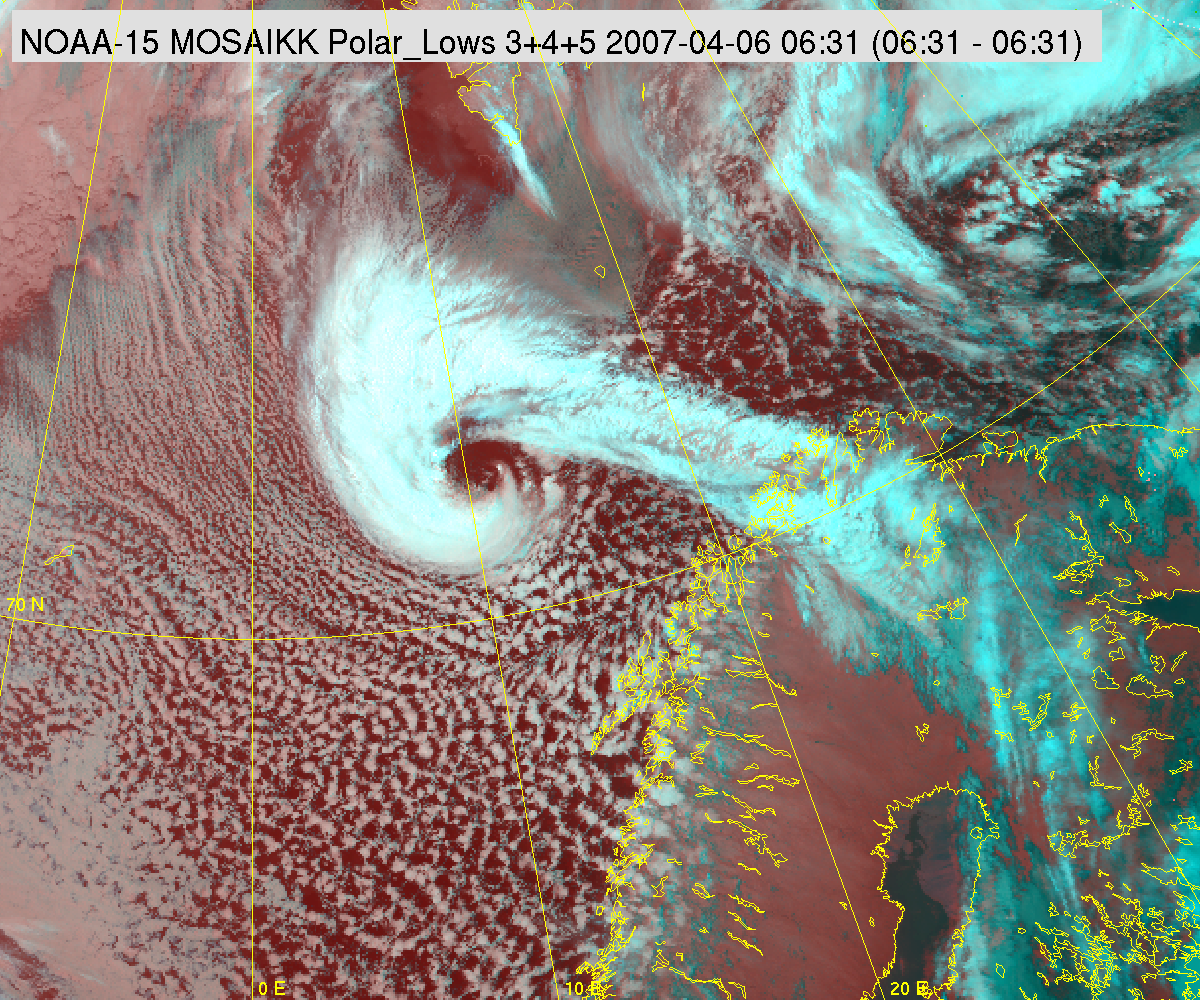
\includegraphics[width=0.7\textwidth]{{figures/PL-image_North_case72}.png}
\end{center}
\end{frame}

\begin{frame}{STARS-72 polar low: model results}
\begin{center}
{\small Pseudo-satellite (TOA OLR) images with SLP contours and precipitation}
\par
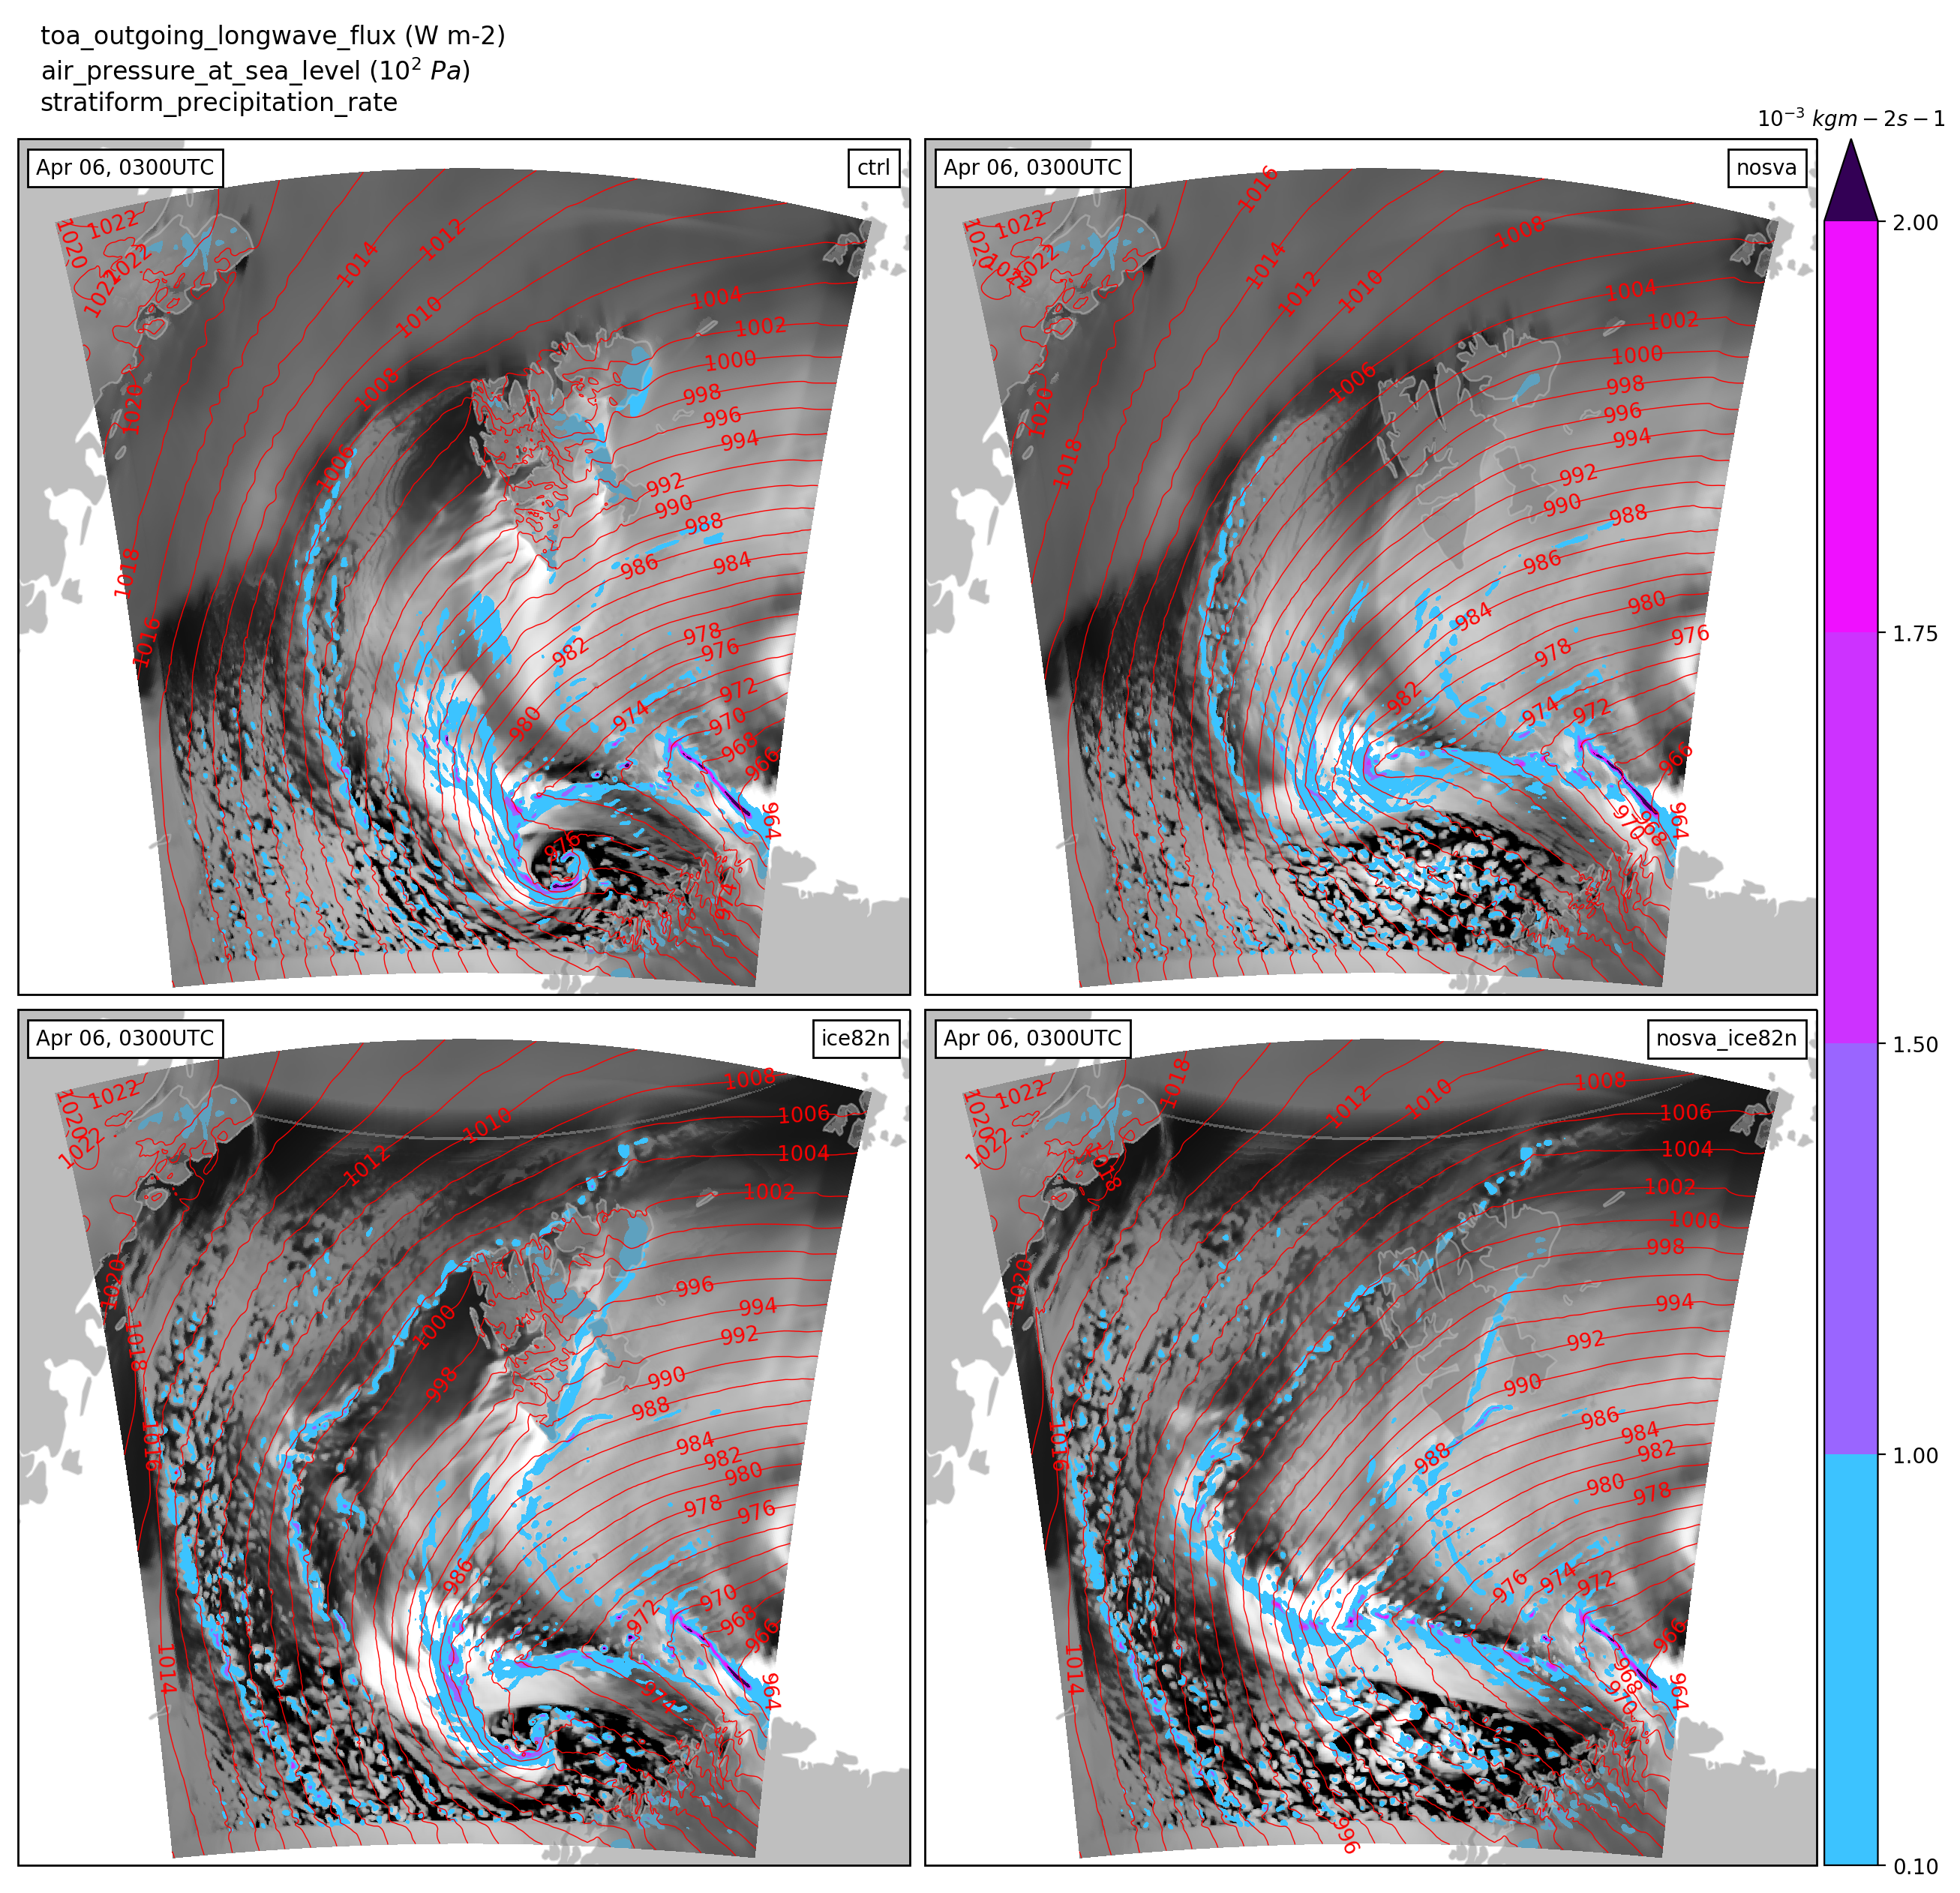
\includegraphics[width=0.7\textwidth]{{figures/lwtoa_slp_precip_cf_20070404T1200Z_km2p2_ctrl_nosva_ice82n_nosva_ice82n_surf_200704060300}.png}
\end{center}
\end{frame}

\begin{frame}{STARS-72 polar low: sensitivity experiments}
\begin{center}
Relative vorticity (\SI{e-4}) at \SI{950}{hPa}: {\Huge 19 h}
\par
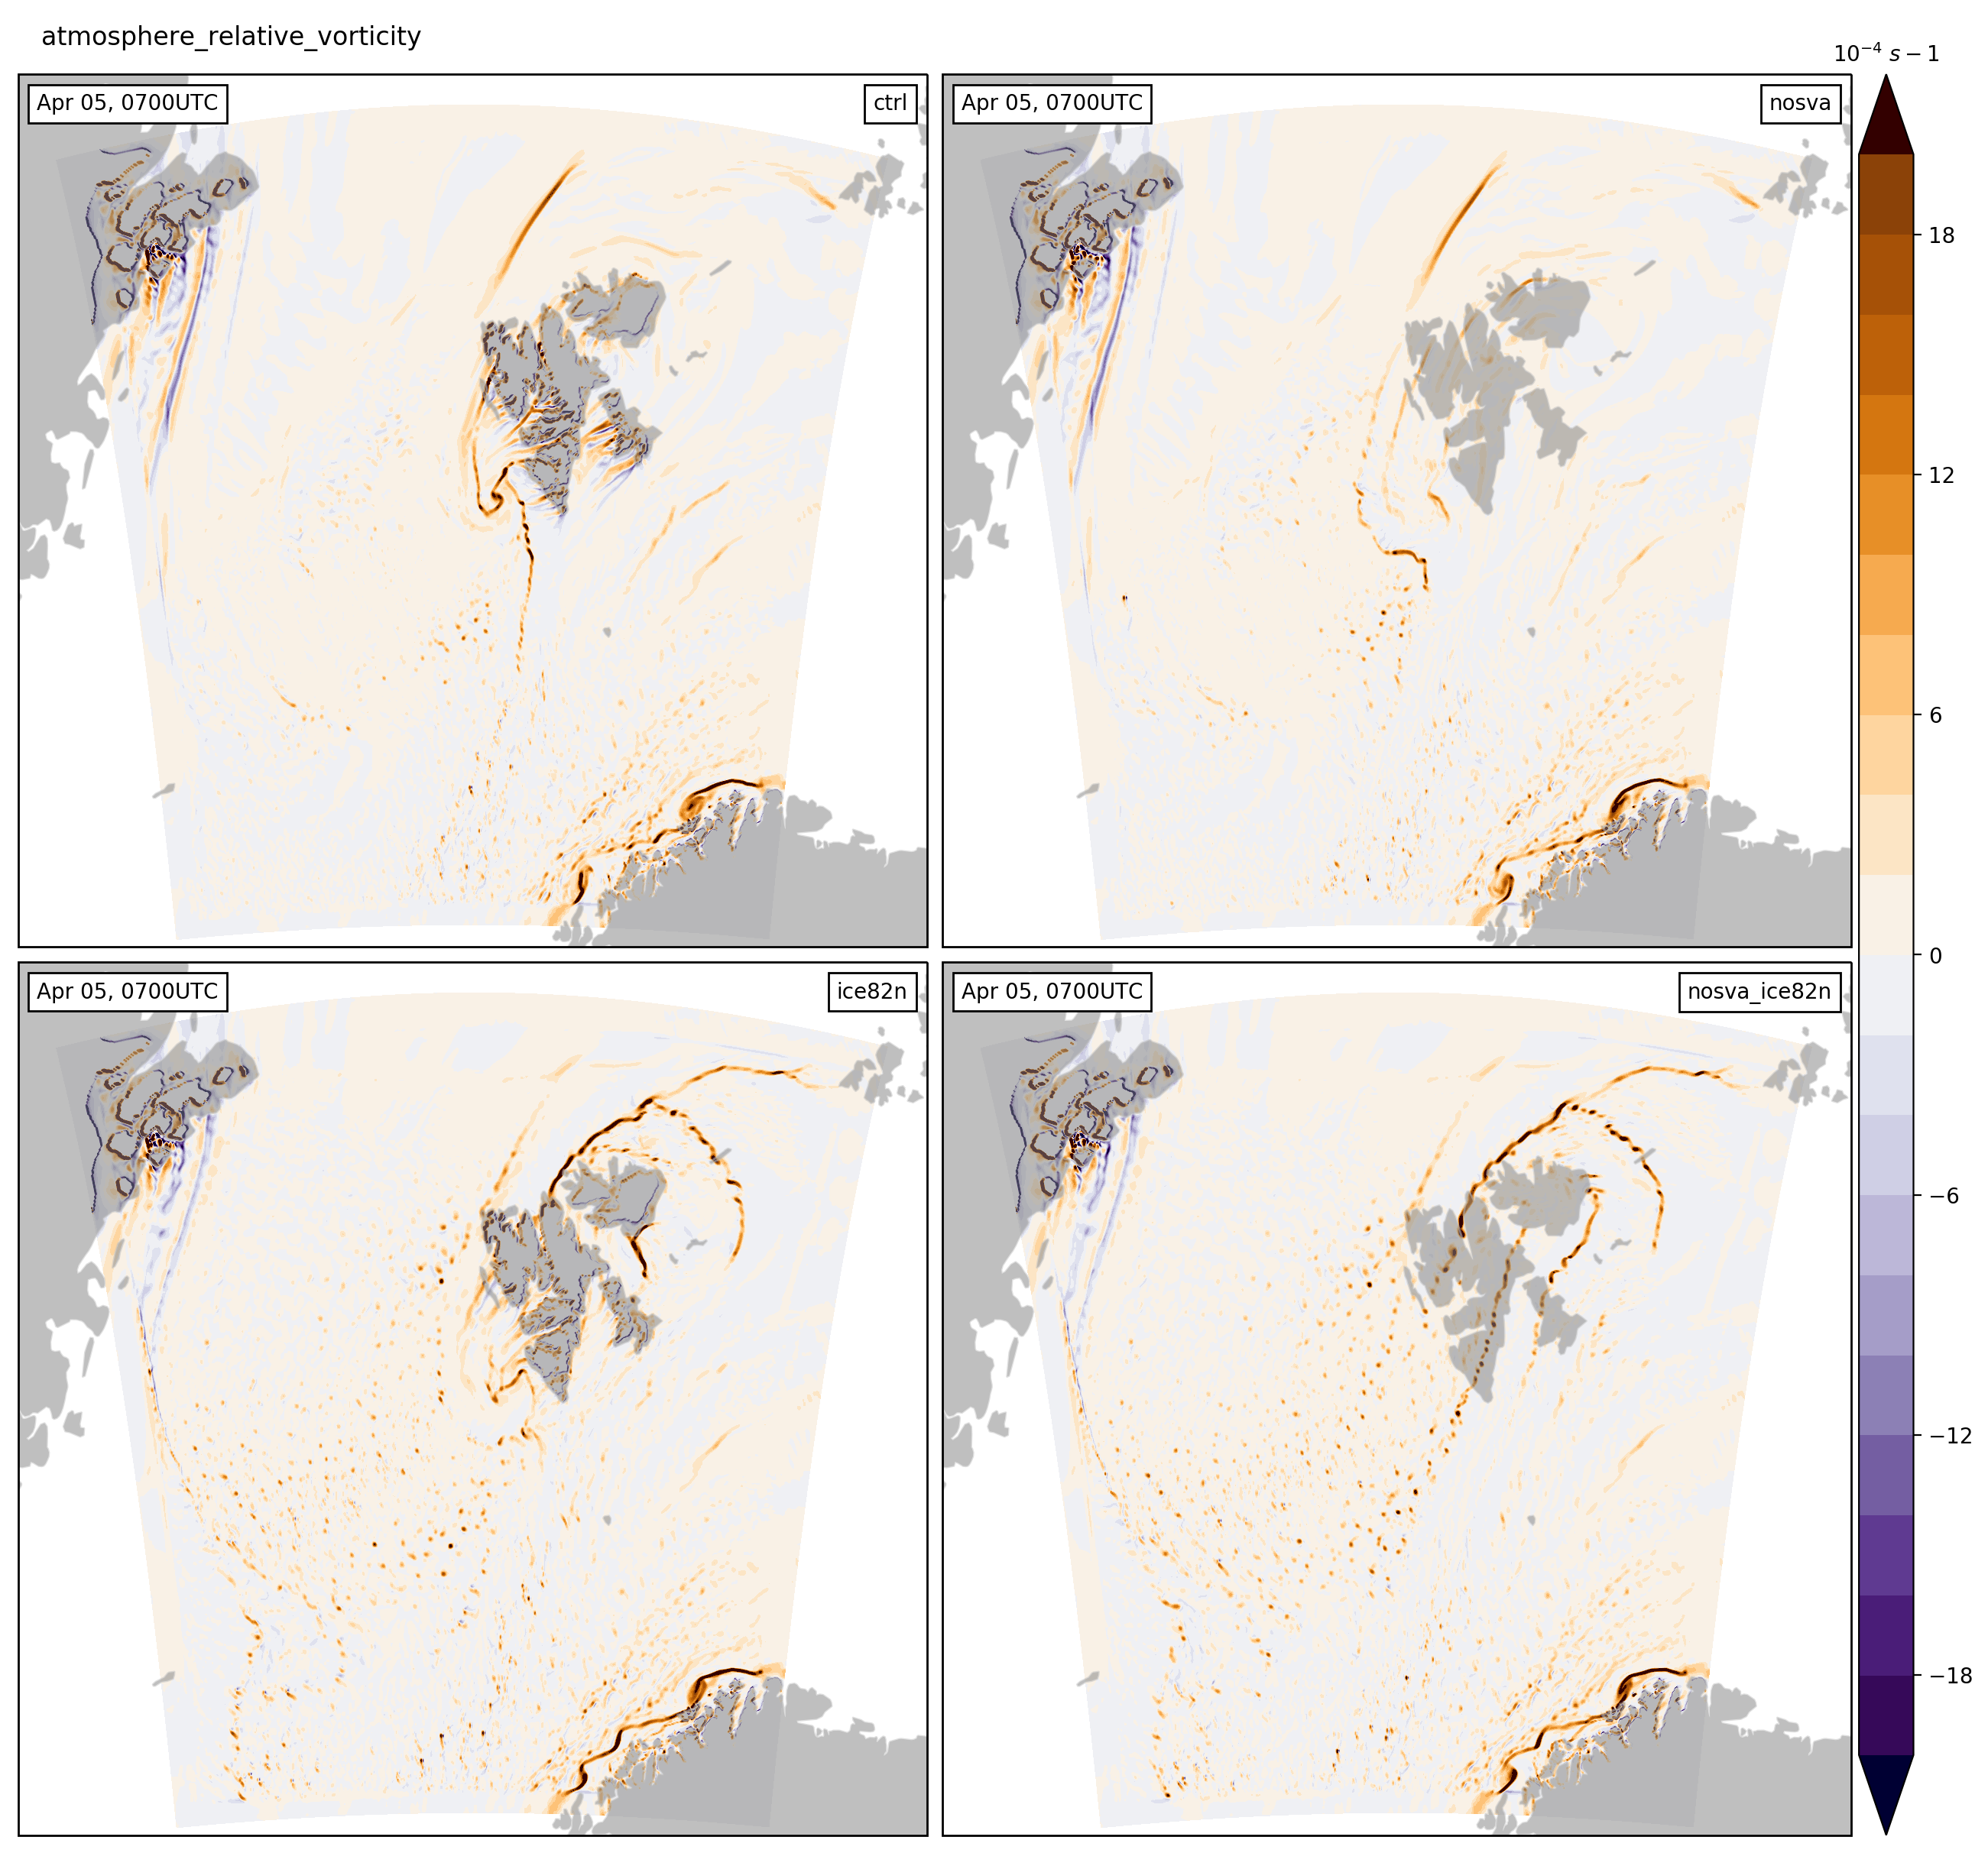
\includegraphics[width=0.7\textwidth]{{figures/vort_cf_20070404T1200Z_km2p2_ctrl_nosva_ice82n_nosva_ice82n_pressure950_200704050700}.png}
\end{center}
\end{frame}

\begin{frame}{STARS-72 polar low: sensitivity experiments}
\begin{center}
Relative vorticity (\SI{e-4}) at \SI{950}{hPa}: {\Huge 33 h}
\par
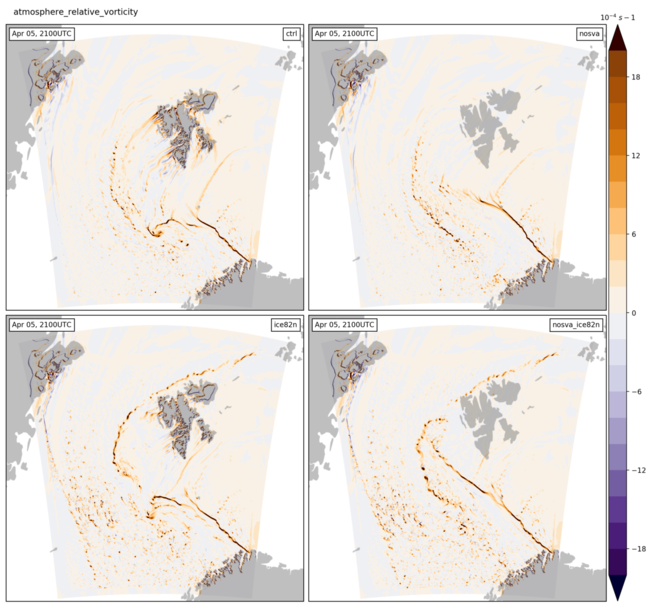
\includegraphics[width=0.7\textwidth]{{figures/vort_cf_20070404T1200Z_km2p2_ctrl_nosva_ice82n_nosva_ice82n_pressure950_200704052100}.png}
\end{center}
\end{frame}

\begin{frame}{STARS-72 polar low: sensitivity experiments}
\begin{center}
Relative vorticity (\SI{e-4}) at \SI{950}{hPa}: {\Huge 39 h}
\par
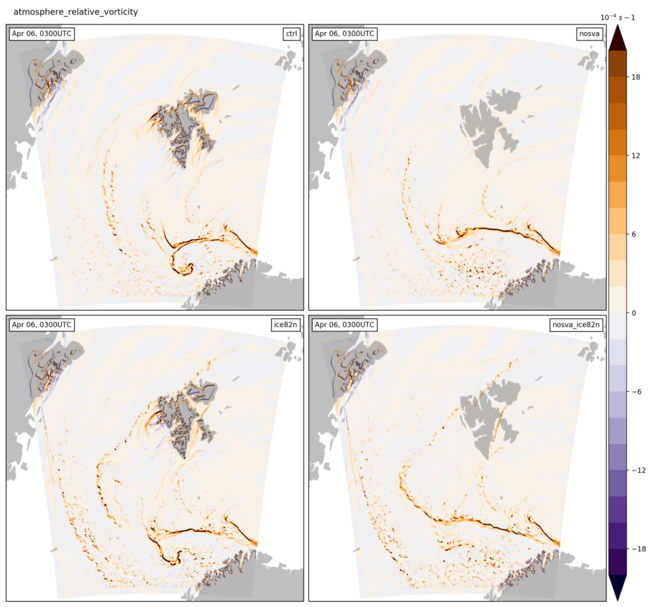
\includegraphics[width=0.7\textwidth]{{figures/vort_cf_20070404T1200Z_km2p2_ctrl_nosva_ice82n_nosva_ice82n_pressure950_200704060300}.png}
\end{center}
\end{frame}

\begin{frame}{STARS-72 polar low: sensitivity experiments}
\begin{center}
Relative vorticity (\SI{e-4}) at \SI{950}{hPa}: {\huge 39 h}
\par
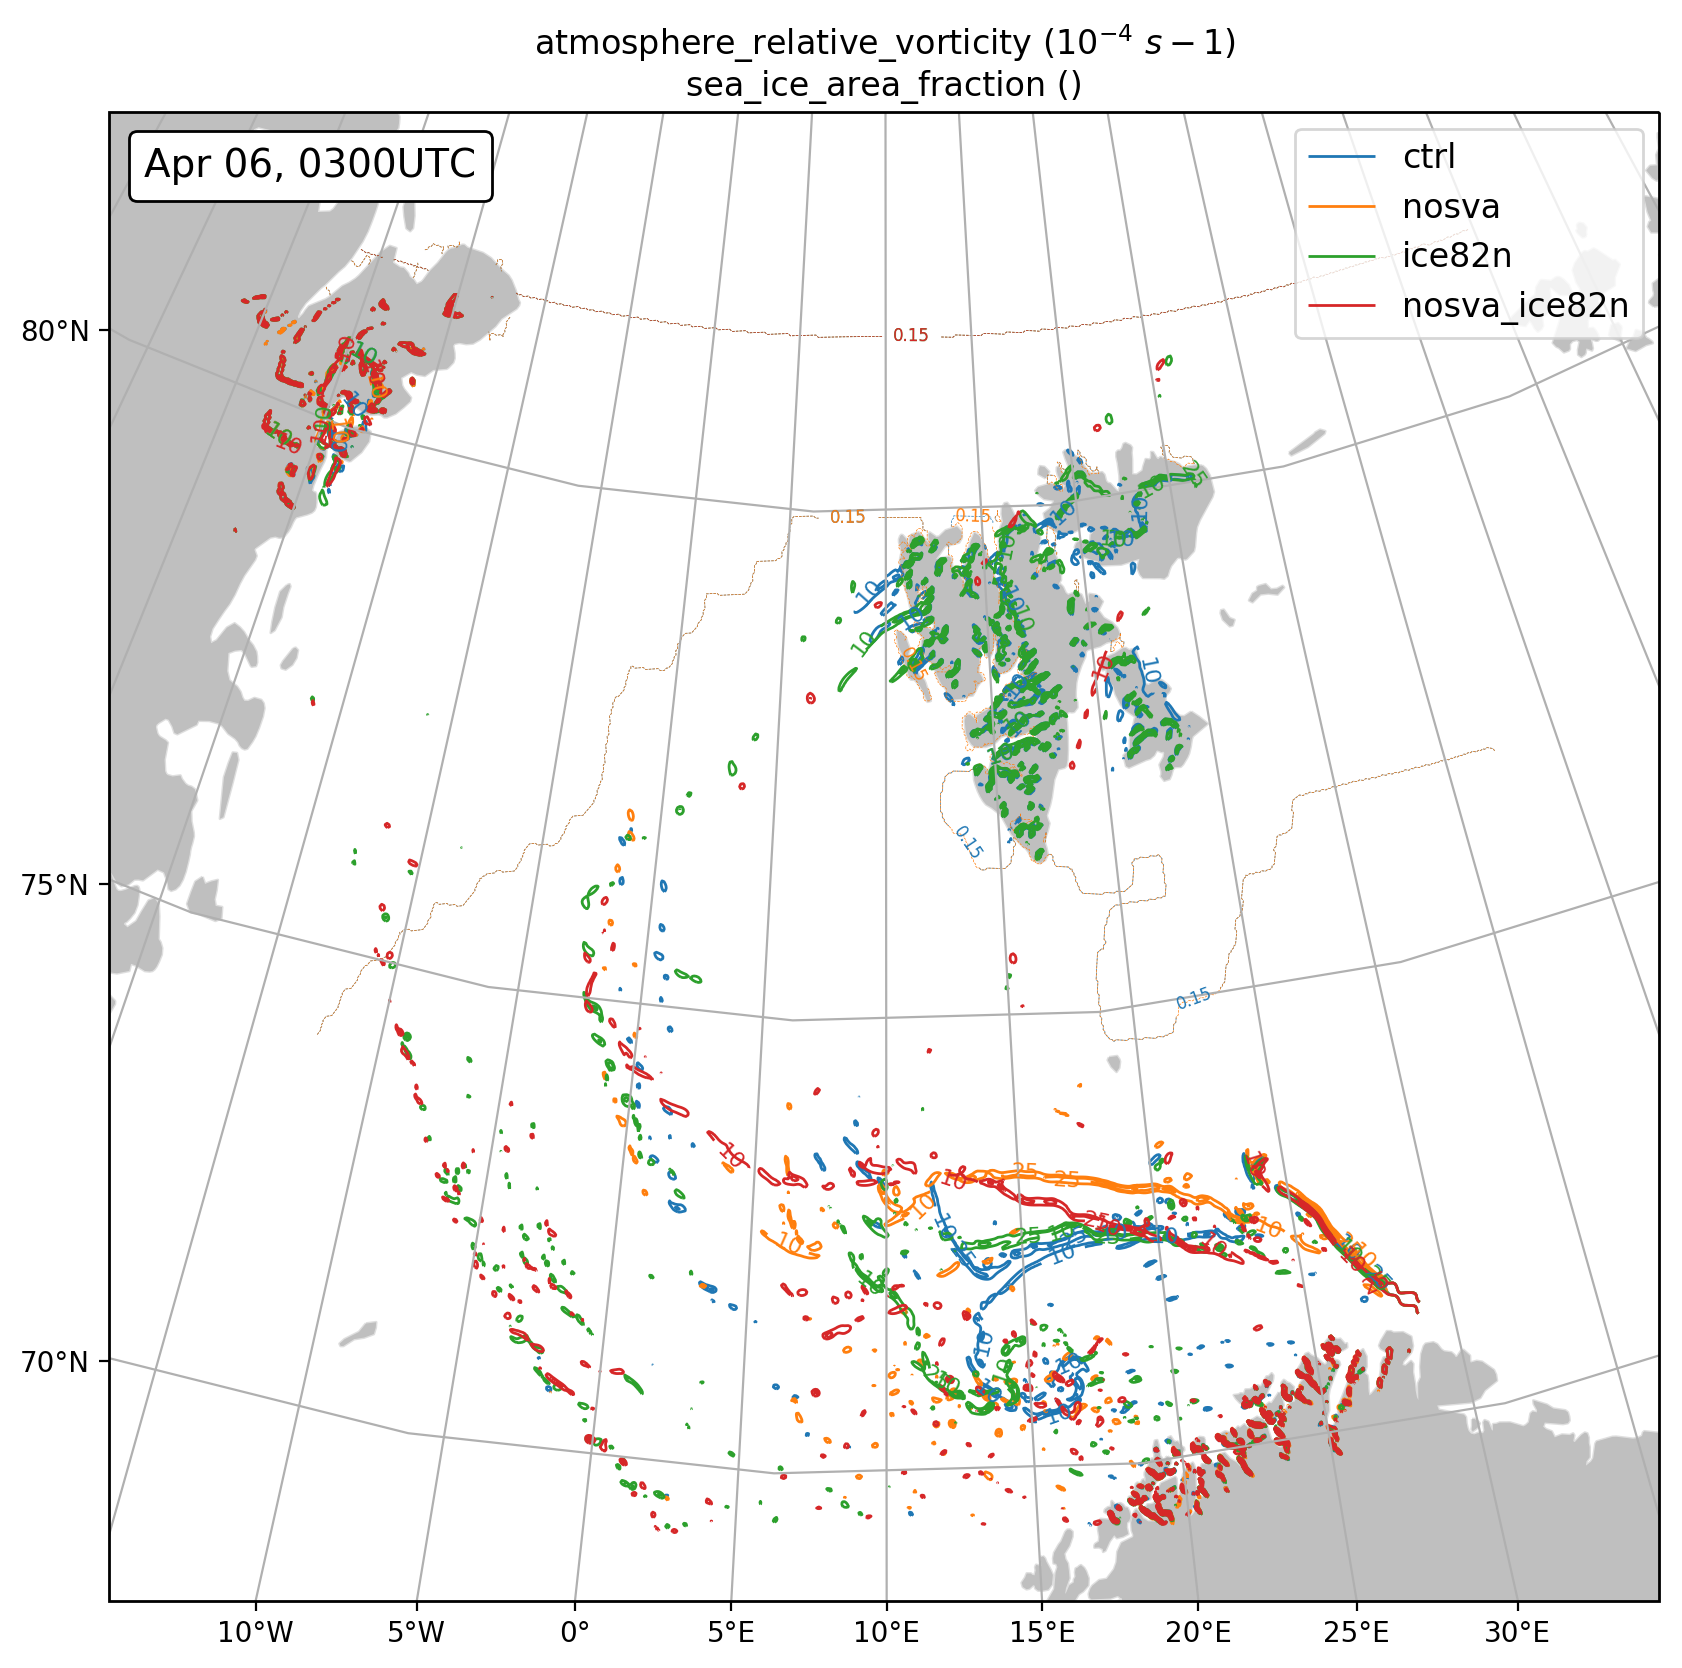
\includegraphics[width=0.7\textwidth]{{figures/vort_diff_20070404T1200Z_km2p2_ctrl_nosva_ice82n_nosva_ice82n_pressure95000_200704060300}.png}
\end{center}
\end{frame}

\section{Another case: STARS-77}
\begin{frame}{STARS-77 polar low}
\begin{center}
AVHRR IR image of polar low event at one selected time
\par
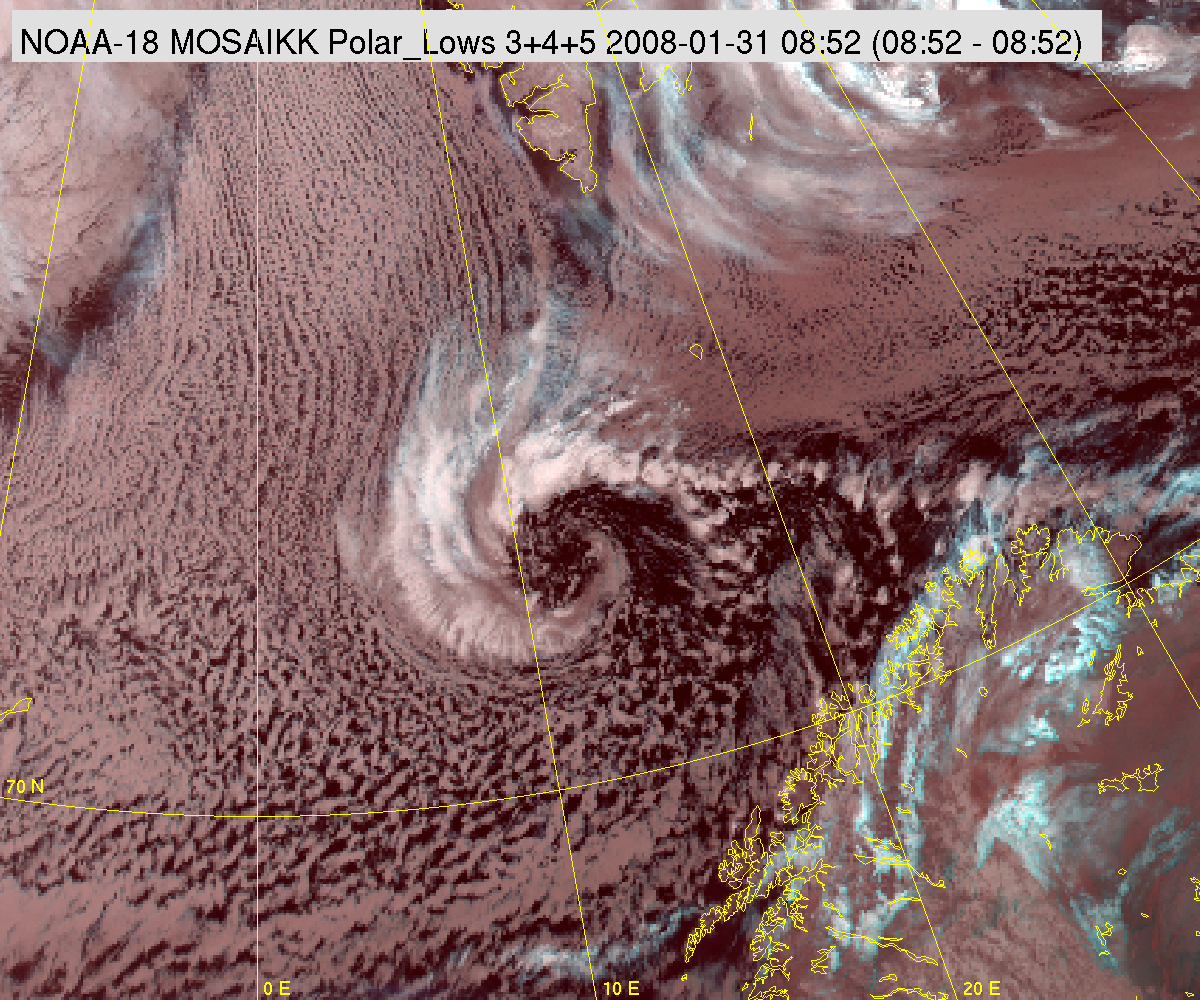
\includegraphics[width=0.7\textwidth]{{figures/PL-image_North_case77}.png}
\end{center}
\end{frame}

\begin{frame}{STARS-77 polar low: sensitivity experiments}
\begin{center}
{\small Pseudo-satellite (TOA OLR) images with SLP contours and precipitation}
\par
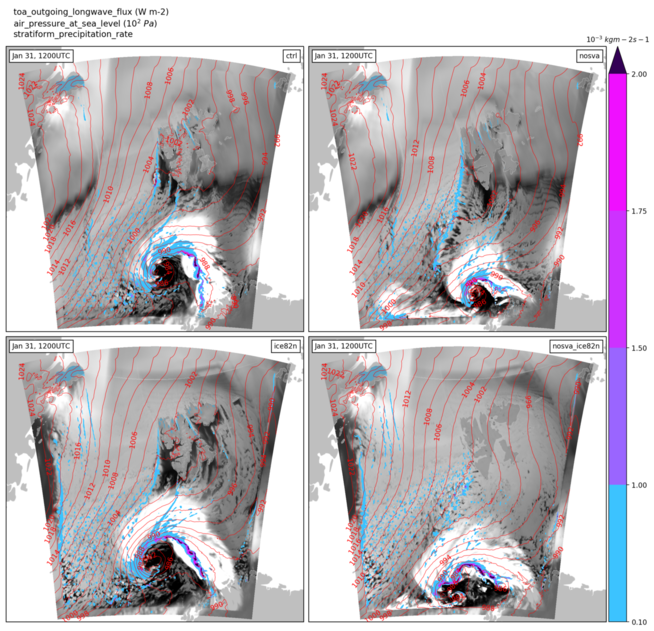
\includegraphics[width=0.7\textwidth]{{figures/lwtoa_slp_precip_cf_20080129T1200Z_km2p2_ctrl_nosva_ice82n_nosva_ice82n_surf_200801311200}.png}
\end{center}
\end{frame}

\begin{frame}{STARS-77 polar low: sensitivity experiments}
\begin{center}
Relative vorticity (\SI{e-4}) at \SI{950}{hPa}: {\huge 30 h}
\par
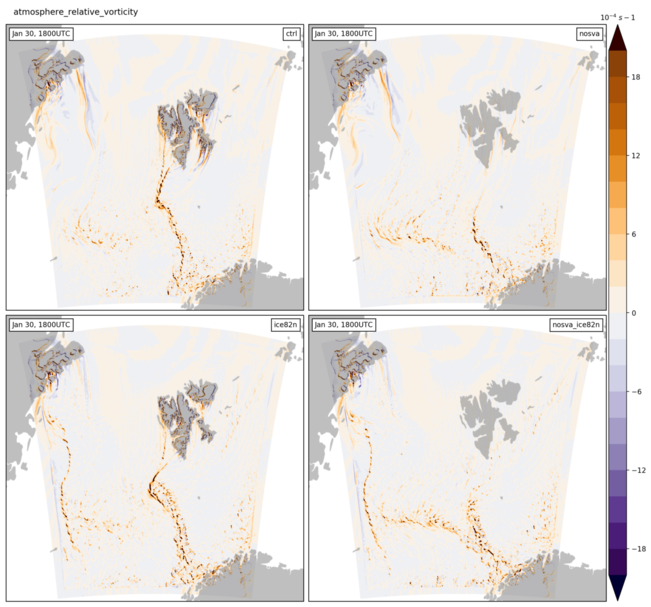
\includegraphics[width=0.7\textwidth]{{figures/vort_cf_20080129T1200Z_km2p2_ctrl_nosva_ice82n_nosva_ice82n_pressure950_200801301800}.png}
\end{center}
\end{frame}
\begin{frame}{STARS-77 polar low: sensitivity experiments}
\begin{center}
Relative vorticity (\SI{e-4}) at \SI{950}{hPa}: {\huge 48 h}
\par
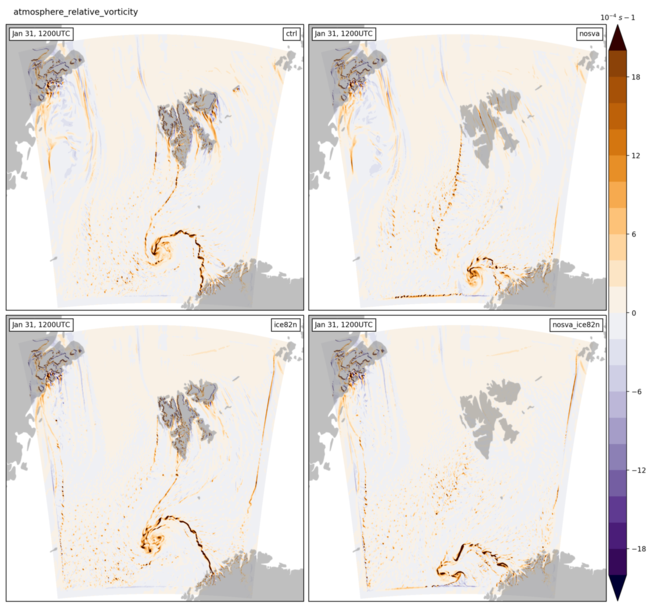
\includegraphics[width=0.7\textwidth]{{figures/vort_cf_20080129T1200Z_km2p2_ctrl_nosva_ice82n_nosva_ice82n_pressure950_200801311200}.png}
\end{center}
\end{frame}


\section{Summary}
\begin{frame}{Some preliminary conclusions}
\begin{itemize}
\item A suite of sensitivity simulations of a real polar low was aimed to understand the role of orography and sea ice
\item The generation of the polar low is resilient and is probably determined by \alert{synoptic-scale flow}
\item The \alert{exact location} and structure is influenced by surface factors
\item Incipient vorticity bands appear in \alert{Svalbard fjords} and are sensitive to orography
\item In other cases, the polar low is only slightly weaker (e.g. STARS-77)
\end{itemize}
\end{frame}

{
\metroset{titleformat frame=allcaps}
\begin{frame}{Thank you!}

{\Huge Questions?}
\vspace{2cm}

\href{mailto:d.sergeev@uea.ac.uk}{\emailsymbol \small{E-mail:} \textbf{d.sergeev@uea.ac.uk}}\\
\href{https://dennissergeev.github.io}{\homepagesymbol \small{Website:} \textbf{dennissergeev.github.io}}\\
\href{http://github.com/dennissergeev}{\githubsymbol \small{GitHub:} \textbf{dennissergeev}}\\
\href{http://twitter.com/meteodenny}{\twittersymbol \small{Twitter:} \textbf{meteodenny}}
\end{frame}
}





% \section{Titleformats}

% \begin{frame}{Metropolis titleformats}
% 	\themename supports 4 different titleformats:
% 	\begin{itemize}
% 		\item Regular
% 		\item \textsc{Smallcaps}
% 		\item \textsc{allsmallcaps}
% 		\item ALLCAPS
% 	\end{itemize}
% 	They can either be set at once for every title type or individually.
% \end{frame}

% {
%     \metroset{titleformat frame=smallcaps}
% \begin{frame}{Small caps}
% 	This frame uses the \texttt{smallcaps} titleformat.

% 	\begin{alertblock}{Potential Problems}
% 		Be aware, that not every font supports small caps. If for example you typeset your presentation with pdfTeX and the Computer Modern Sans Serif font, every text in smallcaps will be typeset with the Computer Modern Serif font instead.
% 	\end{alertblock}
% \end{frame}
% }

% {
% \metroset{titleformat frame=allsmallcaps}
% \begin{frame}{All small caps}
% 	This frame uses the \texttt{allsmallcaps} titleformat.

% 	\begin{alertblock}{Potential problems}
% 		As this titleformat also uses smallcaps you face the same problems as with the \texttt{smallcaps} titleformat. Additionally this format can cause some other problems. Please refer to the documentation if you consider using it.

% 		As a rule of thumb: Just use it for plaintext-only titles.
% 	\end{alertblock}
% \end{frame}
% }

% {
% \metroset{titleformat frame=allcaps}
% \begin{frame}{All caps}
% 	This frame uses the \texttt{allcaps} titleformat.

% 	\begin{alertblock}{Potential Problems}
% 		This titleformat is not as problematic as the \texttt{allsmallcaps} format, but basically suffers from the same deficiencies. So please have a look at the documentation if you want to use it.
% 	\end{alertblock}
% \end{frame}
% }

% \section{Elements}

% \begin{frame}[fragile]{Typography}
%       \begin{verbatim}The theme provides sensible defaults to
% \emph{emphasize} text, \alert{accent} parts
% or show \textbf{bold} results.\end{verbatim}

%   \begin{center}becomes\end{center}

%   The theme provides sensible defaults to \emph{emphasize} text,
%   \alert{accent} parts or show \textbf{bold} results.
% \end{frame}

% \begin{frame}{Font feature test}
%   \begin{itemize}
%     \item Regular
%     \item \textit{Italic}
%     \item \textsc{SmallCaps}
%     \item \textbf{Bold}
%     \item \textbf{\textit{Bold Italic}}
%     \item \textbf{\textsc{Bold SmallCaps}}
%     \item \texttt{Monospace}
%     \item \texttt{\textit{Monospace Italic}}
%     \item \texttt{\textbf{Monospace Bold}}
%     \item \texttt{\textbf{\textit{Monospace Bold Italic}}}
%   \end{itemize}
% \end{frame}

% \begin{frame}{Lists}
%   \begin{columns}[T,onlytextwidth]
%     \column{0.33\textwidth}
%       Items
%       \begin{itemize}
%         \item Milk \item Eggs \item Potatos
%       \end{itemize}

%     \column{0.33\textwidth}
%       Enumerations
%       \begin{enumerate}
%         \item First, \item Second and \item Last.
%       \end{enumerate}

%     \column{0.33\textwidth}
%       Descriptions
%       \begin{description}
%         \item[PowerPoint] Meeh. \item[Beamer] Yeeeha.
%       \end{description}
%   \end{columns}
% \end{frame}
% \begin{frame}{Animation}
%   \begin{itemize}[<+- | alert@+>]
%     \item \alert<4>{This is\only<4>{ really} important}
%     \item Now this
%     \item And now this
%   \end{itemize}
% \end{frame}
% \begin{frame}{Figures}
%   \begin{figure}
%     \newcounter{density}
%     \setcounter{density}{20}
%     \begin{tikzpicture}
%       \def\couleur{alerted text.fg}
%       \path[coordinate] (0,0)  coordinate(A)
%                   ++( 90:5cm) coordinate(B)
%                   ++(0:5cm) coordinate(C)
%                   ++(-90:5cm) coordinate(D);
%       \draw[fill=\couleur!\thedensity] (A) -- (B) -- (C) --(D) -- cycle;
%       \foreach \x in {1,...,40}{%
%           \pgfmathsetcounter{density}{\thedensity+20}
%           \setcounter{density}{\thedensity}
%           \path[coordinate] coordinate(X) at (A){};
%           \path[coordinate] (A) -- (B) coordinate[pos=.10](A)
%                               -- (C) coordinate[pos=.10](B)
%                               -- (D) coordinate[pos=.10](C)
%                               -- (X) coordinate[pos=.10](D);
%           \draw[fill=\couleur!\thedensity] (A)--(B)--(C)-- (D) -- cycle;
%       }
%     \end{tikzpicture}
%     \caption{Rotated square from
%     \href{http://www.texample.net/tikz/examples/rotated-polygons/}{texample.net}.}
%   \end{figure}
% \end{frame}
% \begin{frame}{Tables}
%   \begin{table}
%     \caption{Largest cities in the world (source: Wikipedia)}
%     \begin{tabular}{lr}
%       \toprule
%       City & Population\\
%       \midrule
%       Mexico City & 20,116,842\\
%       Shanghai & 19,210,000\\
%       Peking & 15,796,450\\
%       Istanbul & 14,160,467\\
%       \bottomrule
%     \end{tabular}
%   \end{table}
% \end{frame}
% \begin{frame}{Blocks}
%   Three different block environments are pre-defined and may be styled with an
%   optional background color.

%   \begin{columns}[T,onlytextwidth]
%     \column{0.5\textwidth}
%       \begin{block}{Default}
%         Block content.
%       \end{block}

%       \begin{alertblock}{Alert}
%         Block content.
%       \end{alertblock}

%       \begin{exampleblock}{Example}
%         Block content.
%       \end{exampleblock}

%     \column{0.5\textwidth}

%       \metroset{block=fill}

%       \begin{block}{Default}
%         Block content.
%       \end{block}

%       \begin{alertblock}{Alert}
%         Block content.
%       \end{alertblock}

%       \begin{exampleblock}{Example}
%         Block content.
%       \end{exampleblock}

%   \end{columns}
% \end{frame}

% \begin{frame}{Quotes}
%   \begin{quote}
%     Veni, Vidi, Vici
%   \end{quote}
% \end{frame}

% {%
% \setbeamertemplate{frame footer}{My custom footer}
% \begin{frame}[fragile]{Frame footer}
%     \themename defines a custom beamer template to add a text to the footer. It can be set via
%     \begin{verbatim}\setbeamertemplate{frame footer}{My custom footer}\end{verbatim}
% \end{frame}
% }

% \begin{frame}{References}
%   Some references to showcase [allowframebreaks] \cite{knuth92,ConcreteMath,Simpson,Er01,greenwade93}
% \end{frame}

% \section{Conclusion}

% \begin{frame}{Summary}

%   Get the source of this theme and the demo presentation from

%   \begin{center}\url{github.com/matze/mtheme}\end{center}

%   The theme \emph{itself} is licensed under a
%   \href{http://creativecommons.org/licenses/by-sa/4.0/}{Creative Commons
%   Attribution-ShareAlike 4.0 International License}.

%   \begin{center}\ccbysa\end{center}

% \end{frame}

% \begin{frame}[standout]
%   Questions?
% \end{frame}

% \appendix

% \begin{frame}[fragile]{Backup slides}
%   Sometimes, it is useful to add slides at the end of your presentation to
%   refer to during audience questions.

%   The best way to do this is to include the \verb|appendixnumberbeamer|
%   package in your preamble and call \verb|\appendix| before your backup slides.

%   \themename will automatically turn off slide numbering and progress bars for
%   slides in the appendix.
% \end{frame}

% \begin{frame}[allowframebreaks]{References}

%   \bibliography{demo}
%   \bibliographystyle{abbrv}

% \end{frame}

\end{document}
